\documentclass[12pt]{article}

\usepackage[utf8]{inputenc}
\usepackage[T1]{fontenc}
\usepackage[french]{babel}
\usepackage[top=2cm, bottom=2cm, left=2cm, right=2cm]{geometry}
\usepackage{listings}
\lstset{
	frame=single,
	rulesep=1mm,
	framesep=5mm,
	framerule=1pt,
	xrightmargin=5mm,
	xleftmargin=5mm,
	language=Java,
	basicstyle=\footnotesize,
	numbers=left,
	numberstyle=\normalsize,
	numbersep=7pt,
}

\usepackage{graphicx}

\title{High Level Concept}
\author{Steven \bsc{Gerard}, Corentin \bsc{Raoult}, Loïc \bsc{Tessier}}
\date {14 Novembre 2014}

\begin{document}
\maketitle{}

\section{Présentation}
Il s’agira d’un "tower defense" en 2D vue de dessus avec une part de jeu de rôle. Ce jeu
s'inspirera du jeu "Orc must die". C'est à dire que le joueur aura une phase où il aura le temps
de poser des pièges, des bonus etc. Puis une phase de combat durant laquelle le joueur pourra
lui-même se battre contre les monstres en s'aidant des pièges posés durant la phase précédente.

\section{Caractéristiques}
\subsection{Déroulement du jeu}
Le déroulement du jeu sera divisé en 4 phases comme le montre la figure \ref{Deroulement du jeu}.
\begin{figure}[h]
\begin{center}
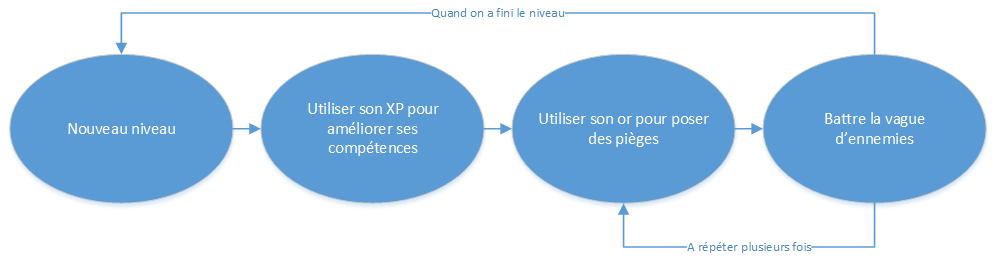
\includegraphics[scale=0.7]{deroulementDuJeu.png} 
\end{center}
\caption{Déroulement du jeu}
\label{Deroulement du jeu}
\end{figure}

\subsection{Capacité des personnages}
Les différents pouvoirs et capacités des personnages multijoueurs sont présentés sur la figure \ref{Capacite des personnages}.
\begin{figure}[h]
\begin{center}
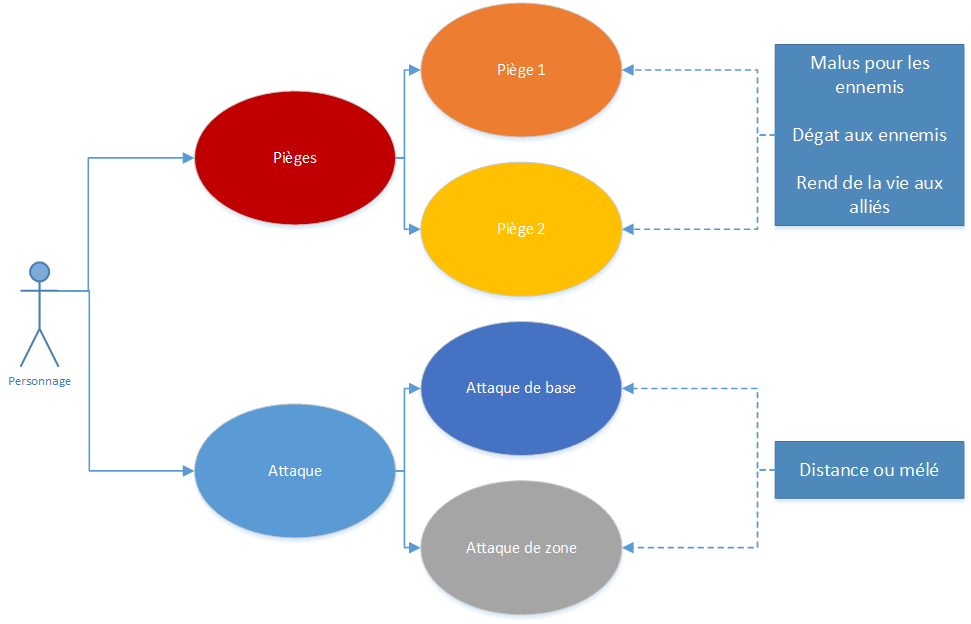
\includegraphics[scale=0.7]{capacite.png} 
\end{center}
\caption{Capacités des personnages}
\label{Capacite des personnages}
\end{figure}
La seule différence pour un joueur solo est qu'il aura accès à tous les pièges.

\pagebreak
\section{Vue d'ensemble}
\subsection{Motivations du joueur}
Le ou les joueurs choisissent un personnage avec certaines caractéristiques propres et doivent essayer de repousser les vagues d'ennemis. Ceci afin de gagner de l'or et des points d'expérience permettant d'améliorer leur personnage au fur et à mesure de la partie.
\subsection{Genre}
Il s'agit d'un "tower defense" avec une phase action/jeu de rôle.
\subsection{Public visé}
Ce jeu s'adresse à des personnes ayant un minimum d'expérience video-ludique mais sans être des "hardcores gamers".
\subsection{Plateforme hardware}
A cause des contrôles à la manette, le jeu s'oriente plus vers les consoles de salon et les PC.
\subsection{Caractéristiques uniques}
Mélange des genres Jeux de rôle, "tower defense" et "beat'em all".
Tower defense coopératif.
\subsection{Compétition}
Ce jeu se joue en coopération et n'est pas en réseau, il n'est donc pas orienté "e-sport"/compétition.


\section{Design}
\subsection{Réflexion}
Le but est de faire réfléchir les joueurs sur une stratégie à adopter pour contrer les vagues d'ennemis lors de la partie "tower defense". La composante jeu de rôle permet aussi de stimuler la réflexion du joueur en lui proposant plusieurs choix d'augmentation des compétences de son personnage.
\subsection{arcade}
Lors de la phase de combat, le jeu se rapproche beaucoup d'un "beat'em all" classique où avoir de bons réflexes est primordial pour faire le meilleur score possible.
\subsection{Coopération}
Lors d'une partie à plusieurs, les joueurs doivent communiquer et réfléchir ensemble afin d'optimiser leur stratégie.
	
\end{document}
